\documentclass[12pt]{article}
\usepackage[utf8]{inputenc}
\usepackage{booktabs}
\usepackage{geometry}
\usepackage{graphicx}
\geometry{a4paper, margin=1in}
\title{Results of the Fisher Combined Test}
\author{Sara Fraija}
\date{\today}
\begin{document}
\maketitle
\section{Resultados}

\begin{table}[h!]
\centering
\resizebox{\textwidth}{!}{%
\begin{tabular}{l c c c c c c}
\toprule
\textbf{GRB} & \textbf{Transit} & \textbf{Significance} & \textbf{Significance Corregida} & \textbf{p-value} & \textbf{Corrected p-value} & \textbf{PDF} \\ \midrule
GRB170708046 & 1__plus_20 & 1.45 & 0.87 & 9.265e-01 & 1.912e-01 & 8.606e-01 \\
GRB170816599 & 1__plus_20 & 1.54 & 0.98 & 9.382e-01 & 1.623e-01 & 8.781e-01 \\
GRB170222209 & 1__plus_20 & 0.86 & -0.79 & 8.051e-01 & 7.860e-01 & 7.244e-01 \\
GRB170403583 & 1__plus_20 & 2.23 & 1.49 & 9.871e-01 & 6.811e-02 & 9.668e-01 \\
GRB170826369 & 1__plus_20 & 1.93 & 0.85 & 9.732e-01 & 1.984e-01 & 9.380e-01 \\
GRB190515190 & 1__plus_20 & 0.63 & -1.55 & 7.357e-01 & 9.396e-01 & 6.729e-01 \\
GRB150101270 & 1__plus_20 & 1.84 & 1.84 & 9.671e-01 & 3.288e-02 & 9.266e-01 \\
GRB150101641 & 1__plus_20 & 1.96 & 1.96 & 9.750e-01 & 2.500e-02 & 9.416e-01 \\
GRB150110923 & 1__plus_20 & 0.34 & 0.34 & 6.331e-01 & 3.669e-01 & 6.235e-01 \\
GRB150120123 & 1__plus_20 & 2.70 & 2.70 & 9.965e-01 & 3.467e-03 & 9.896e-01 \\
GRB150922234 & 1__plus_20 & 0.87 & 0.87 & 8.078e-01 & 1.922e-01 & 7.268e-01 \\
GRB151228129 & 1__plus_20 & 0.61 & 0.61 & 7.291e-01 & 2.709e-01 & 6.688e-01 \\
GRB151229285 & 1__plus_20 & 0.58 & 0.58 & 7.190e-01 & 2.810e-01 & 6.628e-01 \\
GRB160612842 & 1__plus_20 & 0.00 & -0.00 & 5.000e-01 & 5.000e-01 & 6.011e-01 \\
GRB160624477 & 1__plus_20 & 1.17 & 1.17 & 8.790e-01 & 1.210e-01 & 7.988e-01 \\
GRB160726065 & 1__plus_20 & 1.72 & 1.72 & 9.573e-01 & 4.272e-02 & 9.091e-01 \\
GRB170318644 & 1__plus_20 & 0.85 & 0.85 & 8.023e-01 & 1.977e-01 & 7.220e-01 \\
GRB170325331 & 1__plus_20 & 0.94 & 0.94 & 8.264e-01 & 1.736e-01 & 7.435e-01 \\
GRB170803729 & 1__plus_20 & 0.97 & 0.97 & 8.340e-01 & 1.660e-01 & 7.508e-01 \\
GRB170817529 & 1__plus_20 & 0.34 & 0.34 & 6.331e-01 & 3.669e-01 & 6.235e-01 \\
GRB180204109 & 1__plus_20 & 0.00 & -0.00 & 5.000e-01 & 5.000e-01 & 6.011e-01 \\
GRB180418281 & 1__plus_20 & 1.03 & 1.03 & 8.485e-01 & 1.515e-01 & 7.653e-01 \\
GRB180715755 & 1__plus_20 & 0.32 & 0.32 & 6.255e-01 & 3.745e-01 & 6.210e-01 \\
GRB180718082 & 1__plus_20 & 0.60 & 0.60 & 7.257e-01 & 2.743e-01 & 6.668e-01 \\
GRB180805543 & 1__plus_20 & 0.08 & 0.08 & 5.319e-01 & 4.681e-01 & 6.023e-01 \\
GRB181125371 & 1__plus_20 & 2.62 & 2.62 & 9.956e-01 & 4.396e-03 & 9.871e-01 \\
GRB190427190 & 1__plus_20 & 0.00 & -0.00 & 5.000e-01 & 5.000e-01 & 6.011e-01 \\
GRB201008443 & 1__plus_20 & 2.28 & 2.28 & 9.887e-01 & 1.130e-02 & 9.703e-01 \\
GRB201214672 & 1__plus_20 & 0.48 & 0.48 & 6.844e-01 & 3.156e-01 & 6.445e-01 \\
GRB210323918 & 1__plus_20 & 0.51 & 0.51 & 6.950e-01 & 3.050e-01 & 6.497e-01 \\
GRB211024065 & 1__plus_20 & 2.21 & 2.21 & 9.864e-01 & 1.355e-02 & 9.653e-01 \\
GRB220412713 & 1__plus_20 & 1.81 & 1.81 & 9.649e-01 & 3.515e-02 & 9.225e-01 \\
GRB220418720 & 1__plus_20 & 1.19 & 1.19 & 8.830e-01 & 1.170e-01 & 8.035e-01 \\
GRB220511571 & 1__plus_20 & 2.75 & 2.75 & 9.970e-01 & 2.980e-03 & 9.909e-01 \\
GRB220617772 & 1__plus_20 & 0.43 & 0.43 & 6.664e-01 & 3.336e-01 & 6.363e-01 \\
GRB221120895 & 1__plus_20 & 0.04 & 0.04 & 5.160e-01 & 4.840e-01 & 6.014e-01 \\
GRB230228244 & 1__plus_20 & 1.63 & 1.63 & 9.484e-01 & 5.155e-02 & 8.943e-01 \\
GRB230512269 & 1__plus_20 & 1.42 & 1.42 & 9.222e-01 & 7.780e-02 & 8.544e-01 \\
GRB230812790 & 1__plus_20 & 1.41 & 1.41 & 9.207e-01 & 7.927e-02 & 8.524e-01 \\
GRB150819440 & 2__plus_20 & 1.30 & 0.69 & 9.032e-01 & 2.463e-01 & 8.286e-01 \\
GRB170708046 & 2__plus_20 & 0.68 & -0.12 & 7.517e-01 & 5.474e-01 & 6.834e-01 \\
GRB170816599 & 2__plus_20 & 1.98 & 1.52 & 9.761e-01 & 6.486e-02 & 9.438e-01 \\
GRB170206453 & 2__plus_20 & 2.01 & 0.97 & 9.778e-01 & 1.650e-01 & 9.471e-01 \\
GRB170222209 & 2__plus_20 & 0.72 & -1.05 & 7.642e-01 & 8.522e-01 & 6.921e-01 \\
GRB170403583 & 2__plus_20 & 0.10 & -1.81 & 5.398e-01 & 9.651e-01 & 6.030e-01 \\
GRB170826369 & 2__plus_20 & 0.00 & -2.69 & 5.000e-01 & 9.965e-01 & 6.011e-01 \\
GRB190515190 & 2__plus_20 & 0.00 & -2.92 & 5.000e-01 & 9.982e-01 & 6.011e-01 \\
GRB200605762 & 2__plus_20 & 0.60 & -0.59 & 7.257e-01 & 7.226e-01 & 6.668e-01 \\
GRB141205337 & 2__plus_20 & 0.31 & 0.31 & 6.217e-01 & 3.783e-01 & 6.198e-01 \\
GRB150101270 & 2__plus_20 & 0.00 & -0.00 & 5.000e-01 & 5.000e-01 & 6.011e-01 \\
GRB150101641 & 2__plus_20 & 0.31 & 0.31 & 6.217e-01 & 3.783e-01 & 6.198e-01 \\
GRB150922234 & 2__plus_20 & 1.95 & 1.95 & 9.744e-01 & 2.559e-02 & 9.404e-01 \\
GRB151229285 & 2__plus_20 & 0.57 & 0.57 & 7.157e-01 & 2.843e-01 & 6.609e-01 \\
GRB160612842 & 2__plus_20 & 0.00 & -0.00 & 5.000e-01 & 5.000e-01 & 6.011e-01 \\
GRB160624477 & 2__plus_20 & 0.00 & -0.00 & 5.000e-01 & 5.000e-01 & 6.011e-01 \\
GRB160726065 & 2__plus_20 & 1.85 & 1.85 & 9.678e-01 & 3.216e-02 & 9.279e-01 \\
GRB170318644 & 2__plus_20 & 0.26 & 0.26 & 6.026e-01 & 3.974e-01 & 6.143e-01 \\
GRB170325331 & 2__plus_20 & 0.78 & 0.78 & 7.823e-01 & 2.177e-01 & 7.057e-01 \\
GRB170803729 & 2__plus_20 & 0.36 & 0.36 & 6.406e-01 & 3.594e-01 & 6.261e-01 \\
GRB170817529 & 2__plus_20 & 2.24 & 2.24 & 9.875e-01 & 1.255e-02 & 9.675e-01 \\
GRB171007498 & 2__plus_20 & 0.44 & 0.44 & 6.700e-01 & 3.300e-01 & 6.379e-01 \\
GRB180204109 & 2__plus_20 & 0.00 & -0.00 & 5.000e-01 & 5.000e-01 & 6.011e-01 \\
GRB180402406 & 2__plus_20 & 1.10 & 1.10 & 8.643e-01 & 1.357e-01 & 7.821e-01 \\
GRB180418281 & 2__plus_20 & 2.16 & 2.16 & 9.846e-01 & 1.539e-02 & 9.613e-01 \\
GRB180715755 & 2__plus_20 & 1.78 & 1.78 & 9.625e-01 & 3.754e-02 & 9.182e-01 \\
GRB180718082 & 2__plus_20 & 0.67 & 0.67 & 7.486e-01 & 2.514e-01 & 6.813e-01 \\
GRB180805543 & 2__plus_20 & 0.70 & 0.70 & 7.580e-01 & 2.420e-01 & 6.877e-01 \\
GRB181125371 & 2__plus_20 & 1.41 & 1.41 & 9.207e-01 & 7.927e-02 & 8.524e-01 \\
GRB190427190 & 2__plus_20 & 1.97 & 1.97 & 9.756e-01 & 2.442e-02 & 9.427e-01 \\
GRB200415367 & 2__plus_20 & 0.88 & 0.88 & 8.106e-01 & 1.894e-01 & 7.291e-01 \\
GRB201008443 & 2__plus_20 & 1.44 & 1.44 & 9.251e-01 & 7.493e-02 & 8.585e-01 \\
GRB201214672 & 2__plus_20 & 1.78 & 1.78 & 9.625e-01 & 3.754e-02 & 9.182e-01 \\
GRB210323918 & 2__plus_20 & 1.58 & 1.58 & 9.429e-01 & 5.705e-02 & 8.855e-01 \\
GRB210618072 & 2__plus_20 & 1.26 & 1.26 & 8.962e-01 & 1.038e-01 & 8.196e-01 \\
GRB220412713 & 2__plus_20 & 0.65 & 0.65 & 7.422e-01 & 2.578e-01 & 6.770e-01 \\
GRB220418720 & 2__plus_20 & 1.91 & 1.91 & 9.719e-01 & 2.807e-02 & 9.356e-01 \\
GRB220511571 & 2__plus_20 & 0.99 & 0.99 & 8.389e-01 & 1.611e-01 & 7.556e-01 \\
GRB220617772 & 2__plus_20 & 1.83 & 1.83 & 9.664e-01 & 3.362e-02 & 9.252e-01 \\
GRB221120895 & 2__plus_20 & 1.43 & 1.43 & 9.236e-01 & 7.636e-02 & 8.565e-01 \\
GRB230228244 & 2__plus_20 & 0.17 & 0.17 & 5.675e-01 & 4.325e-01 & 6.068e-01 \\
GRB230512269 & 2__plus_20 & 1.76 & 1.76 & 9.608e-01 & 3.920e-02 & 9.152e-01 \\
GRB230812790 & 2__plus_20 & 2.03 & 2.03 & 9.788e-01 & 2.118e-02 & 9.492e-01 \\
\bottomrule
\end{tabular}%
}
\caption{Lista de GRBs with sus Transits, Significances, Significances Corregidas, p-values, p-values Corregidos y valores PDF.}
\end{table}

\begin{figure}[h!]
\centering
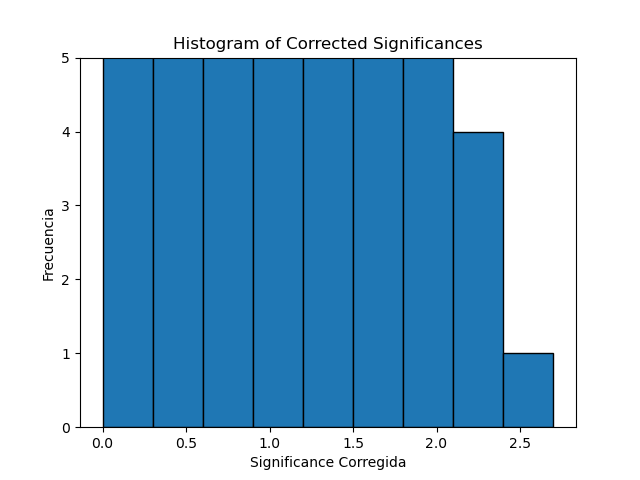
\includegraphics[width=0.6\textwidth]{corrected_significance_hist.png}
\caption{Histogram of Corrected Significances.}
\end{figure}

\section*{Conclusion}
The Fisher combined test integrates individual p-values to evaluate a global hypothesis.
The resulting test statistic was $X^2 = 326.340$ with 164 degrees of freedom.
For a significance level of 0.05, the critical value is 194.883.
Since $X^2$ is greater than the critical value, we rechazamos the null hypothesis of independence.
Normal approximation: p-value = 9.610e-13, significance ≈ 7.04 sigma.

\end{document}